\chapter{Swarm Intelligence}
\section{Introduction}
We stand a lot to gain in Artificial Intelligence by studying the underlying inner workings of nature itself; this is why there is a branch of Artificial Intelligence which incorporates some of nature’s processes, like Genetics, which can be seen in action in the Genetic Algorithm.

 There are other approaches in Artificial Intelligence which also have their routes in Nature, like Animal Learning /Dog Learning.  These approaches only look at a “single agent” thought process when it maps percepts (senses) to actions in its respective environment \cite{DLearning}. 

Swarm Intelligence is an approach more concerned with the underlying processes and behavior patterns when multiple agents (insects, animals) come together and perform a task as one collective entity.  This study of animals or insects in groups has already contributed to Artificial Intelligence as a whole \cite{ChaoticSwarmIntel,BeeJobShop}. Each individual in the swarm might not be able to solve the problem on his own, but by interacting with other individuals and performing primitive actions, the individual can contribute to solving the problem as a whole entity \cite{BeeJobShop}. 

New algorithms which incorporate the lessons learned from the study of the collective intelligence are now being used and form part of the Meta-heuristic algorithm group. The initial algorithms developed with regard to Swarm Intelligence, where based on the coordination and behavior exhibited by schools of fish and flocks of birds. The newer generation of algorithms include\cite{SwarmArt,ChaoticSwarmIntel,BeeJobShop}:
\begin{itemize}
\item Ant Colony Optimization
\item Artificial Bee Colony Optimization.
\item Particle Swarm Optimization 
\end{itemize}

These newer generations of algorithms are primarily being used in combinatorial NP-Complete problems, where there is no defined solution, only an optimization that comes close to a solution. Swarm Intelligence works on a key feature observed in nature, the notion of emergent behavior. Whenever an entity does something unconventional and gains success, it can be considered as exhibiting “Emergent behavior” as if it is emerging out of the masses way of doing things\cite{SwarmArt,CompuIntelligenceIntro}. 

Typical emergent properties exhibited by Swarms are self-organization and synchronization \cite{SwarmArt}. In Swarm Intelligence, when an agent exhibits emergent behavior, the behavior of the agent propagates through the whole swarm.  The behaviour progrates from one agent to another through social interaction which brings forth information exchange \cite{SwarmArt}. Therefore, the whole swarm adapts to a new way of doing things through information that was shared by one agent. The information can be anything that contributes to the swarm as a whole, like for instance the information might be about a new solution that is better than all previous solutions \cite{SwarmArt}. 

Social interaction is but one component of self-organization. Other components that form part of self-organization are \cite{SwarmArt}:
\begin{itemize}
\item positive and negative feedback
\item increasing the magnitude of fluctuations
\end{itemize}
This is why Ant Colony Optimization, Particle Swarm Optimization and Artificial Bee Colony Optimization work so well in NP-Complete problems. The swarm always moves to a better state than previously observed.

NP-Hard optimization problems are only one of the fields of applicability for Swarm Intelligence. Other fields where Swarm Intelligence is being applied include neural network training, network routing, clustering\cite{AntSwarmClustering} , search engines and load balancing \cite{}. Swarm Intelligence thus seems more suited towards problems with combinatorial complexity (B. Denby, 2003).

In this chapter the first discussion will first on Ant Colony Optimization in section~\ref{sec:ACO}. Particle Swarm Optimization will be discussed in section~\ref{sec:PSO}. This chapter will conclude with section~\ref{sec:BEE} where a discussion on the Bee Colony Algorithm will be presented. 

Each section is divided into 3 subsections. First, an overview of the algorithm will be given, where basic concepts about the algorithm will be discussed as well as a general outline of the search process the algorithm uses. The second sub section will give an in depth discussion on some of the core characteristics that make the algorithm unique. Each section will conclude with a literate review of the algorithm being applied on the FAP.

\section{Ant Colony Optimization (ACO)}
\label{sec:ACO}
\begin{figure}[p]
	\begin{center}
	\fbox{\includegraphics[width=5.0in,height=5.5in]{./pictures/AntColonyOptimization.pdf}}
	\caption{Flow Chart for ACO Algorithm}
	\label{fig:ACOAlgorithmFlowChart}
	\end{center}
\end{figure}
\subsection{Overview}
\label{sec:ACOverview}
Ant Colony Optimization is a class of algorithms incorporating different aspects that ants exhibit when they perform certain activities i.e, gather food, build nests and construct cemeteries. The first ACO algorithms that were developed were based on the foraging behaviour that was exhibited by ants when finding the most optimal path towards a food source. The foraging behaviour was noticed by Deneubourg when he performed the Bridge experiment \cite{AntsAndStigmergy,CompuIntelligenceIntro}.
\begin{figure}[b!]
	\centering
	\setlength \fboxsep{0pt}
	\setlength \fboxrule{0.5pt}
	\fbox{\includegraphics[width=4.0in,height=2.0in]{./pictures/antBridgeExperiment.png}}
	\caption{The Ant bridge experiment \cite{AntsAndStigmergy}}
	\label{fig:antBridgeExperiment}
\end{figure}

Deneubourg seeked to know how ants where able to find the shortest path towards a food resource and communicate it to the whole nest \cite{AntsAndStigmergy}. Thus an experiment was setup up to study the ants behaviour. In the experiment a food source was placed a certain distance away from the nest. Two paths were setup towards the food resource, one path was purposely made longer than the other path as can bee seen in figure \ref{fig:antBridgeExperiment} \cite{AntsAndStigmergy}.

The ants would then go out of the nest to gather food for their colony and would in order to do so need to take one of the provided paths toward the food source. What J.L Deneubourg found was that the ants would initially oscillate between the bridges with no clear distinction of the more dominant route to take to retrieve food. But after a certain amount of time more and more ants would start preferring the path which is the shortest path towards food \cite{AntsAndStigmergy}.

Naturally the questioned that was asked was how were the ants able to communicate to each other that the one food source was closer than the other? The answer lies in the use of \emph{stigmergy} \label{def:stigmergy} by ants. Stigmergy is defined as the method animals and insects use to facilitate communication through interaction. Interaction occurs through signals that the individuals receive which might require them to perform a specific action \cite{AntsAndStigmergy,CompuIntelligenceIntro,AntIntroTrends}.

Two forms of stigmergy can be observed in nature. The one form , \emph{Sematectonic stigmergy} \label{def:sematectonic}, is a direct and physical form of interaction since it relies on altering the environment or by using some for of physical action to communicate \cite{CompuIntelligenceIntro}. Examples of this type of stigmergy include nest building and brood sorting \cite{CompuIntelligenceIntro}. 

The other form, \emph{Sign-based stigmergy} is an indirect form of interaction, where communication occurs through some sort signal mechanism \cite{CompuIntelligenceIntro}. Ants use sign-based stigmergy when they are retrieving food. As the ant moves their path is reinforced with a chemical signal that alerts other ants to the desirability of the path \cite{CompuIntelligenceIntro}. The chemical signal that ants use to indicate optimal paths is called \emph{pheromones}.  The concept of pheromones is a critical concept of ACO hence, we will we will provide an in depth discussion on pheromones in sub section \ref{sec:ACOcharacter}.

The ACO algorithms are considered stochastic search procedures due to their innate use of randomness when exploring the solution space \cite{ACOSurvey,ImpACOComplex}.The ACO class of algorithms has been applied to a wide range of problems that include --- INSERT EXAMPLES. The algorithm does have some disadvantages. One of the primary disadvantages of ACO is that it tends to get stuck on local minima in the solution space therefore, the solution space isn't adequately explored and the algorithm prematurely converges to a local optima \cite{ImpACOComplex}.

Improving the exploration of a population of agents in Swarm Intelligence algorithms is no easy feat, especially for the Ant System which uses positive feedback(Gang Wang, 2005). To combat this shortcoming the MAX-MIN Ant Optimization algorithm was developed. The MAX-MIN algorithm is based on the original Ant system algorithm. MAX-MIN addresses the local minima problem by imposing dynamically changing bounds on the pheromones of the ants such that it is always with limit of the heuristic and best current path of the colony (Gang Wang, 2005).

The first algorithm to be based on the behaviour of ants was called the Ants System (AS) \cite{CompuIntelligenceIntro,AntIntroTrends}. The AS was initially applied to the Traveling Salesman problem (TSP) as a proof of concept application, but its performance was lacklustre compared to other algorithms applied to the same problem \cite{CompuIntelligenceIntro,AntIntroTrends}. Subsequently, various algorithms have been developed that improve on the AS. These improved algorithms include the Ant Colony System (ACS), The ANTS system, Ant-Q and AntTabu \cite{CompuIntelligenceIntro,AntIntroTrends}. Where applicable reference to these algorithms will be made to indicate how the have improved the AS system.

In this sub section an overview of the ACO algorithm was given. A discussion was presented on how the algorithm was developed from observing ants. Furthermore a discussion was also presented on how the algorithm utilizes the core communication concept used my ants, called pheromones, is used to search the solution space. In conclusion a small indication of of the typical problems at which ACO excels at as well as some of the disadvantages the algorithm has in its standard form was given.

In the next section a more in depth discussion on the core characteristics of the ACO will be given as well as additional characteristics that were developed in response to improve the efficiency of the algorithm.
\subsection{ACO characteristics}
\label{sec:ACOcharacter}
In this section various characteristics which are important and unique to the ACO class of algorithms will be discussed. A discussion on each of the following characteristics will be discussed (in order of discussion): Pheromones, State Transition Rules and Pheromone evaporation.
\subsubsection{Pheromones trail}
\label{sec:pheromonetrail}
The pheromone technique used by ants forms part of the core methodology used by the Ant Colony Optimization (ACO) algorithm \cite{AntQAP}. As an ant moves it lays down pheromones to mark the path it is walking. Pheromones decay over time therefore, as the ant follows the pheromone trail it reinforces the pheromone that is already on a path \cite{AntQAP}.Thus the more ants following a path the stronger the pheromone trail for that path and the stronger the pheromone the higher probability is that an ant will follow the path \cite{AntQAP}. 

The pheromone reinforcement is the last phase the algorithm enters before continuing to the next iteration as seen in figure \ref{fig:ACOAlgorithmFlowChart}.

In the bridge experiment the ants started following the shorter path, because an ant following the shorter path would reinforce its pheromone trail faster than on the longer path. Initially, the ants oscillated between the two paths since there was no clear indication to the colony what the shortest path was, therefore the ants initially randomly selected the paths they would follow \cite{AntQAP}. Once a path as been marked with pheromones the ant no longer selects a path based solely on randomness. Instead the ant selects a path based on a probability transition rule \cite{AntsAndStigmergy}. Transition rules will be discussed in the next sub section.

With the use of pheromones ants are able to communicate the best and shortest path. The more ants following a preferred path the more pheromones would be laid on that specific path and in return increase the strength of the pheromones \cite{ImpACOComplex}. The increase in strength of the pheromones on a path would thus let ants more clearly distinguish between paths it “should” and “should not” take \cite{ImpACOComplex}. Therefore, a pheromone provides positive feedback to the colony.

When the algorithm starts there are no pheromones to indicate path and the ants are placed at certain positions which are problem dependent. Initially, all the ants will choose random paths. After all the ants have completed their paths, each path is evaluated\cite{CompuIntelligenceIntro}. The amount of pheromone marking a path is in the standard ACO related to the cost function. Therefore, a low cost function value will have a high pheromone dosage indicating the path the ant took from each node and a high cost function value will have a low dosage\cite{CompuIntelligenceIntro}. 

The pheromone of each path hence, allows the colony to remember good and bad decisions from previous iterations\cite{CompuIntelligenceIntro}. This is a form of local pheromone updating \label{def:localpheromoneupdate}which will be discussed in the pheromone update section. In the iterations following the initial one, the ants will at each node decide based on a probability function whether it should follow the pheromone trail laid down in previous iterations or choose a new path to another node. Thus as the ACO iterates through more iterations the stronger particular path pheromone trail will become, hence signalling the path out as the best found \cite{CompuIntelligenceIntro}.


The pheromone trail was initially developed with only one colony in mind \cite{CompuIntelligenceIntro}. In the research done by Tiwari et al. pheromones in multiple colonies are considered. The basic principle of how pheromones are used by the ants stays the same, but the meaning of the pheromone changes if an ant of another colony encounters the pheromone trail. The ant will not follow or even consider the pheromone trail since any pheromone encountered from other colonies repulse the ant. Thus pheromones only provide positive feedback if the ant is from the same colony, otherwise the pheromone gives negative feedback, in a way warning the ant to stay away. This repulsion strategy promotes exploration among the multiple colonies  \cite{ACOLargeProblem}.

In this section we gave an in depth discussion on what pheromones are as well as how they are applied in the most basic of cases. In the next sub section we will discuss the different transition rules that each algorithm in the class of ACO algorithms use.
\subsubsection{State transition rules}
 As discussed in the previous sub section the ants select which path next to follow based on a probability. This probability is also known as the \emph{transition probability}. In this sub section we will provide some of transition probabilities in use. Pheromone trails is the core concept upon which the Ant System is based and was the first algorithm developed based on ants that used the pheromones concept\cite{CompuIntelligenceIntro}. 
\begin{equation}
\label{eq:ASprobability}
p^k_{ij}(t) =
\begin{cases}
	\frac{\tau^{\alpha}_{ij}(t)\eta^{\beta}_{ij}}{\sum_{u \in N^k_i(t)} {\tau^{\alpha}_{iu}(t)\eta^{\beta}_{iu}(t)}}, &\text{if $j \in N^k_i(t)$}\\
	0, &\text{if $j \notin N^k_i(t)$}\\
\end{cases}
\end{equation}
The first transition probability is formulated in equation (\ref{eq:ASprobability}) and is used by individual ants of the AS algorithm \cite{CompuIntelligenceIntro,AntSurvey}. An ant $k$ uses this equation to decide with what probability it will move from a node $i$ to a node $j$ \cite{CompuIntelligenceIntro}. $\tau_{ij}$ is the amount pheromone that exists between the path linking node $i$ and $j$ \cite{CompuIntelligenceIntro,AntsAndStigmergy}. Heuristic information is incorporated into the equation through the symbol $\eta_{ij}$ which is the desirability of the path from node $i$ to node $j$ as evaluated by an heuristic function \cite{CompuIntelligenceIntro,AntsAndStigmergy}. 

As can been observed from the figure \ref{fig:ACOAlgorithmFlowChart}, the algorithm individually moves each ant based on these defined transition probabilities.

Through the use of parameters $\alpha$ to represent pheromone intensity and $\beta$ to represent heuristic information the algorithm is able to achieve a good balance between exploration and exploitation when $\alpha=\beta$ \cite{CompuIntelligenceIntro}. When $\alpha = 0$ no pheromone is taken into account, hence, any history that the algorithm has on the path between node $i$ and node $j$ is neglected and the algorithm degrades to a stochastic greedy search procedure. If $\beta = 0$ then the algorithm does not take into account the amount of desirability the path between node $i$ and node $j$ as dictated by the problem specific heuristic function.

The set $j \in N^k_i(t)$ contains all the valid neighborhood moves ant $k$ is allowed to make when moving from node $i$ to node $j$. A tabu list is kept by each ant to trim the set of moves already performed previously, hence cycling is prevented.

Various other algorithms have been developed that improve on the basic AS. Each algorithm uses a different transition probability equation that might be very specific to the domain or a slight variant of the above equation as with the Ant Colony System. This section is not intended to give an exhaustive survey of different transition rules that exist in the literate. Therefore, we only discuss the first transition rule developed since most other rules can simply be considered derivatives of the basic transition rule.
\subsubsection{Pheromone update}
As discussed in the pheromone section, pheromones start to evaporate \footnote{Pheromone evaporation is discussed on page \pageref{sec:pheromoneevapuation}}over time hence, the path marked by the pheromone trail becomes less attractive to the ants. Therefore, a path that represents a good solution needs its pheromone trail to be continuously updated. In this sub section we will discuss the rules that govern when and by how much pheromones are updated.

 Most of the variants that have been developed differ in the sense of what pheromone update rules they employ. In the literature pheromone update rules are classified into two groups \cite{CompuIntelligenceIntro}. The one group is called the global update rule. The other group is called the iteration based or local update rule of which an example has been given on page \pageref{def:localpheromoneupdate} \cite{CompuIntelligenceIntro}. 

The first local pheromone rule was presented in the AS algorithm \cite{CompuIntelligenceIntro}. The ants would retrace their path after each iteration, depositing pheromones on each link that makes the complete path. The following equation was used to update the pheromone:
\begin{align}
 \tau_{ij}(t+1) &= \tau_{ij}(t) + \Delta\tau_{ij}(t),\\ 
 \text{where }\Delta\tau_{ij} &= \sum^{n_k}_{k=1}\Delta\tau^k_{ij}(t) \notag
\end{align}
Pheromone update rules that are in the global update group, only allow the pheromone trail of the path representing the best found solution by the algorithm since the first iteration, to be updated \cite{CompuIntelligenceIntro}. Thus the global rule favours intensification where the algorithm exploits the global knowledge gained by the ants to find a better solution. By updating we mean the pheromone is reinforced. 

The Ant Colony System (ACS) was the first to use the global update rule together with the local update rule\cite{CompuIntelligenceIntro}. By using both types of rules the algorithm is able to efficiently exploit the history provided by the pheromones\cite{CompuIntelligenceIntro}. The global update rule used by the ACS is formulated in the following equation\cite{CompuIntelligenceIntro}:
\begin{align}
	\tau_{ij}(t + 1) &= (1 - p_1)\tau_{ij}(t) + p_1\Delta\tau_{ij}(t),\\
	\text{where }\Delta\tau_{ij} &= \notag
	\begin{cases}
		\frac{1}{f(x^+(t))} &\text{if $(i,j) \in x+(t)$}\\
		0 &\text{otherwise}
	\end{cases}
\end{align}
The parameter $x+(t)$ represents the best / shortest path so far found by the algorithm\cite{CompuIntelligenceIntro}. The rest of the parameters represents the same concepts as discussed on page \pageref{eq:ASprobability}

As can been seen in the following equation, the ACS uses a slight variant of the local update rule first used in AS\cite{CompuIntelligenceIntro}.
\begin{equation}
	\tau_{ij}(t) = (1 - p_2)\tau_{ij} + p_2\tau_0
\end{equation}
In the above equation $\tau_0$ is a small constant and $p_2 \in [0,1]$ is the constant that defines the rate of evaporation\cite{CompuIntelligenceIntro}.

This phase of the algorithm, is executed as the very last step as can be observed from figure \ref{fig:ACOAlgorithmFlowChart}

\subsubsection{Pheromone evaporation}
\label{sec:pheromoneevapuation}
Initially when the pheromone concept was first implemented the ants of the colony rapidly converged on a solution and did not adequately search the solution space for alternate path that might lead to better solutions. To combat this premature convergence and force the ants to explore the solution space more, the concept of \emph{pheromone evaporation} was introduced\cite{CompuIntelligenceIntro,AntsAndStigmergy,AntIntroTrends,AntSurvey}. 

As discussed in the pheromone sub section (see \pageref{sec:pheromonetrail}) the pheromone marking a trail evaporates over time until it is reinforced by an ant. The evaporation of pheromones is governed by equation \ref{eq:pheromoneevapuration}\cite{CompuIntelligenceIntro,AntsAndStigmergy,AntIntroTrends,AntSurvey}:
\begin{equation}
\label{eq:pheromoneevapuration}
	\tau_{ij}(t) \leftarrow (1-p)\tau_{ij}(t), p\in [0,1]
\end{equation}
The constant $p$ defines the rate at which pheromone evaporates. If $p=1$ the pheromone completely evaporates every iteration and the ants take no history into account with regard to there path selection and the search is completely random \cite{CompuIntelligenceIntro,AntsAndStigmergy}. Thus, the amount of exploration done by the algorithm can be controlled with the constant $p$ \cite{CompuIntelligenceIntro,AntsAndStigmergy}.

The above equation (\ref{eq:pheromoneevapuration}) was first introduced in the Ant System \cite{CompuIntelligenceIntro,AntsAndStigmergy,AntIntroTrends,AntSurvey}. Most subsequent algorithms that are form of the ACO class of algorithms also use the concept of pheromone evaporation, but they either use the standard equation or develop their own variant \cite{CompuIntelligenceIntro,AntsAndStigmergy,AntIntroTrends,AntSurvey}.

% Content in "A new solution algorithm for improving performance of ant colony optimization"
A more aggressive form of Pheromone evaporation  is add to the Ant system discussed in the research done by \cite{AntQAP}. The more aggressive form works beside the already present pheromone evaporation, instead this form seeks to add an additional search phase called \emph{diversification}. 

In the ant system developed by the authors a mechanism is added that monitors a certain number of solutions that have been recently produced. If the solution hasn't changed a certain number of iterations the mechanism removes all pheromone trails currently in the system. 

Therefore, the algorithm is forced to re-search the search space to create new solutions as it cannot rely on previous historic information provided by the pheromone trails. This mechanism forces the algorithm to diversify \cite{AntQAP}.

As can be observed from the figure \ref{fig:ACOAlgorithmFlowChart} the last phase is where all the pheromone laid by the ants are updated for the next iteration. Pheromone evaporation forms part this phase.
\subsection{ACO on the FAP}
As discussed in the overview section \ref{sec:ACOverview} the ACO has been applied to a wide number of problems and has produced good results. Thus, the ACO has also been applied to the FAP instance of problems.

In research presented by Luna et. al\cite{ACOvsEA} an ACO algorithm is presented and applied to a custom cellular network instance. The custom cellular network instance the authors use has 711 sectors with 2,612 tranceivers which need to be assigned frequencies. For their particular network, only 18 channels are available for assignment. The channels start at 134 and end at 151\cite{ACOvsEA}.

The authors presented two versions of the algorithm. The one version uses no heuristic information (hence forth referred to as ACO*) and the other version uses heuristic information to update the pheromone laid done by the artificial ants\cite{ACOvsEA}.

With regard to the heuristic updating the pheromone trails, the authors opted to increase the pheromone by some magnitude\cite{ACOvsEA}. This magnitude was hand tuned to be 100. The heuristic only increases a certain paths pheromone if the frequencies assigned to the transceivers this path represents differ enough as to not cause significant interference\cite{ACOvsEA}. Thus, the heuristic aims to amplify good choices made previously by the algorithm for the next iteration of the algorithm.

The results the authors obtained will now be presented for both versions of the algorithm that was developed\cite{ACOvsEA}.

\begin{center}
	\begin{tabular}{| c | c | c |}
	\hline
	Time limit & ACO* & ACO \\ \hline
	120s & 104719.72 & 91140.04 \\ \hline
	600s & 103752.12 & 89703.44 \\ \hline
	1800s & 103781.86 & 88345.94 \\ \hline
	\end{tabular}
\end{center}

The authors note, that if one observed the results they obtained, one can clearly see that the ACO version that incorporates heuristic information to reinforce pheromone trails outperforms the version which doesn't do it\cite{ACOvsEA}. The above values represent the amount of interference which will result if the plan is used in the network\cite{ACOvsEA}.
\section{Artificial Bee Colony Algorithm}
\label{sec:BEE}
\begin{figure}[p]
	\begin{center}
	\fbox{\includegraphics[width=5.0in,height=5.5in]{./pictures/BeeAlgorithm.pdf}}
	\caption{Flow Chart for the BEE Algorithm}
	\label{fig:BeeAlgorithmFlowChart}
	\end{center}
\end{figure}
\subsection{Overview}
The Artificial Bee Colony (ABC) algorithm is the youngest algorithm discussed in this chapter. It was first proposed by Karaboga in 2005 and seeked to mimic the foraging behaviour exhibited by bees \cite{ABCCompareStudy,ABCLeafConstrained,ABCNumericalOptimization}. Like ants, bees need to gather food to support the colony. To understand how the ABC algorithm tries to mimic the foraging behaviour of bees, we first need to explain how real bees forage \cite{ABCCompareStudy}. 

In a bee colony there are a numerous number of bees, each with a specific role that performs certain actions for the colony. There are bees that protect the queen, bees that maintain the colony, bees that scout for resources and finally bees that gather food i.e the worker bees. The most important bees for foraging are those that scout and gather food \cite{ABCCompareStudy}. 

The scout bees are sent out and as their role implies, they are responsible for exploring the surroundings of the hive to find suitable food sources \cite{ABCCompareStudy}. If a food source has been found by scout bee, then it needs to return to the colony to share the information with the worker bees \cite{ABCCompareStudy}. When the bee enters the colony it needs to communicate to the other bees by using some form of stigmergy (see page \pageref{def:stigmergy} \cite{ABCCompareStudy}.

The scout bee accomplishes this communication by performing a dance known as the ``waggle dance'' in the colony for all the bees to see \cite{ABCCompareStudy}. This isn't a dance like in the traditional sense, since through certain movements the bee is able to communicate a variety of characteristics about the food source that include \cite{ABCCompareStudy}:
\begin{itemize}
\item How far the food source is from the colony.
\item Quality of the food source.
\item Path towards the food source.
\end{itemize}

Therefore, it can be concluded that with regard to foraging bees use \emph{Sematectonic} stigmergy (see page \pageref{def:sematectonic}) as the dance is a physical form of communication.

The dance is observed by ``onlooker'' worker bee \cite{ABCCompareStudy,ABCImageEnhancement}. These onlooker bees are currently ``unemployed'' in the colony \cite{ABCCompareStudy,ABCImageEnhancement}. After the information of the scout be has been transferred the onlooker bees, becomes an ``employed'' bee since it is moving to the food source to start gather food \cite{ABCCompareStudy,ABCImageEnhancement}. Thus it is the job of the worker bees to \emph{exploit} the information provided by the \emph{exploration} done by the scout bees \cite{ABCCompareStudy,ABCNumericalOptimization}. 

Worker bees gather food from the designated food source, until the food source reaches a certain quantity with regard to nectar content \cite{ABCCompareStudy,ABCNumericalOptimization}. Each time the bee returns to the colony it evaluates the current food source versus other food sources discovered \cite{ABCCompareStudy,ABCNumericalOptimization}. Hence, if there is better food source found, the bee abandons the previous and starts gathering food from the new source \cite{ABCCompareStudy,ABCNumericalOptimization}. On the other hand, if the food source has been exhausted meaning there is no more nectar content to gather, the bee returns to the colony and becomes ``unemployed'' again \cite{ABCCompareStudy,ABCNumericalOptimization}.

In the ABC algorithm, the food sources are the solutions \cite{ABCCompareStudy,ABCNumericalOptimization}. Each food source has an employed bee associated with it. Onlooker bees either wait for new food sources to be communicated to them or become employed bees by moving to another an attractive food source \cite{ABCCompareStudy,ABCNumericalOptimization}. 

As with real honey bees, a ``waggle dance'' is performed to all the onlooker bees by employed bees which provides information on the nectar amount (fitness value) that they represent \cite{ABCReconfigDistro,ABCCompareStudy,ABCImageEnhancement}. The onlooker bees choose food sources depending on the nectar amount \cite{ABCReconfigDistro,ABCCompareStudy,ABCImageEnhancement}. Therefore as the nectar amount of a food source increases the probability that the more onlooker bees will choose the source increases \cite{ABCReconfigDistro,ABCCompareStudy,ABCImageEnhancement}. The probability will be discussed in the next sub section.

Bees can transition to different roles depending on their situation \cite{ABCCompareStudy,ABCNumericalOptimization}. An onlooker bee becomes employed when assigned to a food sources and a employed bee can become a scout if his initial food source becomes exhausted \cite{ABCImageEnhancement,ABCCompareStudy,ABCReconfigDistro}. Note, that not all employed bees of a food source become scouts, only the first employed bee of a food source transitions to a scout \cite{ABCImageEnhancement,ABCCompareStudy,ABCReconfigDistro}. Scout bees are sent to randomly generated food sources \cite{ABCImageEnhancement,ABCCompareStudy,ABCReconfigDistro}. 

The more onlooker bees a food source attracts, the more the neighbourhood will get explored since the onlooker bees move to the food source and choose an immediate neighbouring food source to be employed upon \cite{ABCCompareStudy,ABCNumericalOptimization}. Thus, this can be considered exploitation and the algorithm is therefore performing a local search. Finally, the number of onlooker bees a food source has also indicates its desirability, hence, a very good solution will have the majority of onlooker bees choosing it and search for nearby better food sources \cite{ABCCompareStudy,ABCReconfigDistro,ABCNumericalOptimization}.

When a food source is abandoned, the previous bee that occupied the food source transitions to a scout bee \cite{ABCCompareStudy,ABCNumericalOptimization}. The scout bee is responsible for replacing the abandoned food source by find a new one, therefore, a new one is generated and communicated back to the colony \cite{ABCCompareStudy,ABCImageEnhancement,ABCNumericalOptimization}. The generation of food sources will be discussed in the next sub section.

Karaboga was not the first to base an algorithm on the above foraging behaviour. In the literature other bee foraging inspired algorithms have been developed such as the BeeHive Algorithm, Bee Colony Optimisation (BCO) and Bee Swarm Optimization (BSO) \cite{BCO,HybridABCClustering,ABCNumericalOptimization}. 

The BeeHive algorithm is based on the dance communication used inside the colony of bees. In BCO solutions are randomly generated and assigned to bees\cite{HybridABCClustering,ABCNumericalOptimization}. The solutions are then progressively modified using certain strategies. Finally BSO solutions are iteratively constructed by forager (worker) bees and the best solution is communicated to the rest of the colony by performing a dance\cite{HybridABCClustering,ABCNumericalOptimization}. All of the above mentioned algorithms were developed to be primarily used on combinatorial problems \cite{ABCCompareStudy}.

Another bee algorithm is the Virtual Bee Algorithm (VBA) which, like the previous algorithms and is also based on the foraging behaviour of bees, but it differs in the sense that it isn't designed for combinatorial problems \cite{ABCNumericalOptimization}. Instead, VBA is designed for numerical function optimization \cite{ABCNumericalOptimization}. In VBA bees would move around in the search space communicating to each other any target nectar food sources that were found \cite{ABCNumericalOptimization}.

Karaboga developed the ABC algorithm based on the previous research done on bee colony optimization and the above algorithms. The ABC algorithm is designed to be a multi-variable optimisation algorithm and has to date been applied to the Job Scheduling Problem, Clustering \cite{HybridABCClustering}, Neural Network training and Reconfiguration of Distribution Networks \cite{ABCReconfigDistro}. Due to the nature of the algorithm being similar to that of the ACO, we can expect the ABC algorithm to be applied to a whole host of problems present in the literature.

In this sub section we gave a brief overview of the Artificial Bee Colony Algorithm. We discussed the real bee behaviour the algorithm tries to recreate and  gave other algorithms that are also based on the same process. Finally, we defined the primary design goal of the algorithm and presented some of the problem on which the algorithm has been applied.

In the next sub section, we will discuss some of the core characteristics of the algorithm.
\subsection{BEE algorithm characteristics}
In this subsection we will discuss the characteristics of the ABC algorithm that define the algorithm and make it unique. We will start of by first explaining how food sources are handled in the algorithm. We will then discuss how information is communicated to the colony. Finally, we will finish off this sub section with a more precise discussion on how foraging in modelled and used in the algorithm.
\subsubsection{Food Sources}
As discussed in the overview, food sources represent solutions to the problem the ABC algorithm is being applied to. When the algorithm starts, there are no defined food sources for the bees to evaluate and report on. Therefore, initially a finite amount of food sources are randomly generated. Since each food source needs an employed bee to evaluate the nectar amount of the source, the parameter that defines the amount of food sources also defines the amount of employed bees.

Employed bees evaluate these food sources by determining their nectar amount. The nectar amount is directly related to the fitness value calculated using a domain specific cost function. After the amount if determined the employed bee advertises the food source to the colony by performing the waggle dance. 

Onlooker bees bear witness to a number of dances from a variety of employed bees. The onlooker bees therefore need to select a food source that is the most attractive while maintaining some diversity in the pool of solutions. Thus, an onlooker bee selects a food source based on a probability function which is formulated in equation (\ref{eq:beeProbability})\cite{ABCCompareStudy}:
\begin{equation}
\label{eq:beeProbability}
p_i = \frac{{fit}_i}{\sum^{SN}_{n=1}{fit}_n}
\end{equation}

The parameter $p_i$ is the $i$th food source under consideration by the onlooker bee. As discussed above, the ${fit}_i$ parameter represents the value of the cost function and is directly related to the nectar amount of food source $i$. The parameter SN is the maximum amount of food source and hence the maximum employed and/or onlooker bees \cite{ABCCompareStudy}.

\subsubsection{Employed and Onlooker Bees}
As outlined in the overview, when recruited onlooker bees reach the advertised food source that is stored in memory, they do not occupy the same food source. Instead, the bees explore the immediate neighbourhood of the food source that communicated to them. The onlooker bees seek to find a food source that improves on the previous one. Equation (\ref{eq:beeGenerate}) is used by the bees to generate new food sources in the neighbourhood of a food source $x_i$.
\begin{equation}
\label{eq:beeGenerate}
v_{ij} = x_{ij} + \phi_{ij}(x_{ij} - x_{kj})
\end{equation}
The subscripts $k \in \{1,2,\dots,SN\}$ and $j \in \{1,2,\dots,D\}$ are indexes which are randomly chosen. $D$ represents the maximum dimensionality of the vector a solution represent. The index $k$ has an constraint tied to it -- whatever value is randomly assigned to $k$ it \emph{must} differ from the value $i$. The position of the new food source in the neighbourhood of $x_{ij}$, is controlled by the $\phi_{ij}$ parameter which is a bounded random value between $[-1,1]$. 

From equation (\ref{eq:beeGenerate} it can be concluded that the randomness of the food source position decreases as the difference between $x_{ij} - x_{kj}$ decreases. Thus, as the algorithm moves closer to an optimal solution the finer grained the search process becomes of the algorithm.

After a new solution $v_i$ is produced, the bee takes the new solution and the old solution from memory to compare their respective nectar contents. If the new solution is found to have higher quality nectar, the bee replaces the old solution in memory with the new solution. Otherwise, the bee abandons the new solution and keeps the old solution in memory. Thus, the bee seeks to always move towards a better solution and therefore, uses a greedy selection process.

One of the problems with the above approach is that little information about the food source is used in generating a neighbouring food source. In the research by Singh \cite{ABCLeafConstrained} a slight variation is proposed to generating food source neighbours by using more global information. The authors add a constraint to the algorithm that all neighbouring solutions generated by \emph{employed} bees must be unique. 

When an employed bee generates a neighbour and a identical solution already exists in the system, a \emph{collision} is said to have occurred. A collision is solved by letting the employed bee transition to a scout bee so that a completely random solution can be generated \cite{ABCLeafConstrained}. Scout and Onlooker bee generated solutions are not checked if it collides with other solutions in the system since the aim for them is exploration and not exploiting like with employed bees. 
\subsubsection{Scout bee}
The artificial bees are modelled to based on the behaviour of real bees. Thus certain food sources can also be abandoned by an employed bee when it has outlived its usefulness. Abandonment of a food source can occur due to the following aspects:
\begin{itemize}
\item The employed bee has reached the maximum allowed cycles to improve the nectar amount. The maximum cycles spends on a food source allows the algorithm to avoid local optima.
\item The solution represented by the food source cannot be improved any further by the bee.
\end{itemize}
When a food source in the algorithm is abandoned, it needs to be replaced with a new food source. An employed bee under goes a role transition when it abandons a food source. The bee transition from an employed bee to a scout bee. 

It is the responsibility of the scout bee to replace the abandoned food source with a new randomly generated one. Scout be uses equation (\ref{eq:scoutGenerate}) to produce new food source that will replace food source $x_i$.
\begin{equation}
\label{eq:scoutGenerate}
x^j_i = x^j_{min} + rand[0,1](x^j_{max} - x^j_{min})
\end{equation}

In research done by G\'{o}mez-Iglesias et. al \cite{ABCFusionGrid} an extension is made to the scout bees. The Scout bee individuals are divided into two types of bees namely \emph{Rovers} and \emph{Cubs} bees\cite{ABCFusionGrid}.
\begin{itemize}
\item{Rover bees} are similar to traditional scout bees and hence use diversification strategies to explore the solution space. 
\item {Cub bees} explore the solution space relative to a good solution found by a Rover through randomly changing configuration parameters. 
\end{itemize}
By using two different scout bees a good balance is achieved when searching the solution space in the beginning where diversity if preferred and late in the algorithm where intensification is preferred \cite{ABCFusionGrid}.
\subsection{BEE algorithm on the FAP}
The BEE algorithm and all its variants are relatively new. The algorithm has for now only been applied to a select few problems such as the Traveling Salesman Problem.

As of yet, no research has been done to apply the BEE algorithm to the FAP. Therefore a possible avenue of future work would be to apply one of the BEE algorithm variants to the FAP.

In the next section a discussion will be presented on the Particle Swarm Optimization algorithm.
\section{Particle Swarm Optimization (PSO)}
\label{sec:PSO}
\begin{figure}[p]
	\begin{center}
	\fbox{\includegraphics[width=5.0in,height=5.5in]{./pictures/ParticleSwarmOptimization.pdf}}
	\caption{Flow Chart for PSO Algorithm}
	\label{fig:PSOAlgorithmFlowChart}
	\end{center}
\end{figure}
\subsection{Overview}
Particle Swarm Optimization (PSO) is a self-adaptive, population-based stochastic search technique that was developed by Kennedy and Ebenhart in 1995 \cite{PSOGABreeding,PSOGABreeding}. The basic model of the algorithm is based on simulations done to recreate the natural behaviour of a flock of birds \cite{PSOSoftTesting}.

In the early stages of the particle swarm development, simulations were developed to closely model the stigmergy (see page \pageref{def:stigmergy}) exhibited when a flock of birds cohesively move as one and is able to suddenly change direction in a unpredictable graceful manner only to regroup as one observed entity \cite{PSOHybridJobShop}. 

As the ``leading'' bird of the flock changes his movements the information is shared to the all birds that are in the immediate neighbourhood of the leading bird. As the information is shared locally among the birds, each bird modifies his own movement to that of the leading birds movement\cite{PSOHybridJobShop}. 

Thus, because birds obtain information through observation of their neighbouring birds, the stigmergy can be deemed of a physical nature. Therefore, the particular stigmergy used by birds is Sematectonic stigmergy (see page \pageref{def:sematectonic}).

The simulations based on this behaviour of the flock, allowed researchers to discover the underlying patterns that governed the way birds are able to share information about the general movement of the flock. Based on these patterns and simulations the particle swarm algorithm emerged into an optimization algorithm \cite{CompuIntelligenceIntro}.

In the algorithm a particle is an individual. A group of particles, referred to in the literature as swarm, fly through the solution space of the problem the algorithm is being applied to. Each particle changes his movement based on information shared to him by neighbouring particles in the swarm \cite{FundamentalSwarm,CompuIntelligenceIntro}. 

As information is shared among particles, the success of one particle ripples through the rest of the swarm and each particle is able to utilize shared information that lead to success of another particle. Thus, each particle own personal experience and knowledge of the search space has an effect on its neighbouring particles \cite{FundamentalSwarm,CompuIntelligenceIntro}.

There exists two primary PSO algorithms called Global PSO and Local PSO. The only difference between the two algorithms are how they go about sharing information to the rest of the swarm. The sharing models of these two algorithms along with other sharing models will be discussed in the PSO characteristics subsection \cite{SOSwarm}.

In the swarm, each particle is a potential solution that is encoded in a D-dimensional vector \cite{PSOHybridJobShop,PSOSelfHierarch}. As a particle moves through the solution space, it continually evaluates its current position and adjusts it accordingly to move in the general direction of the best particle of the swarm. 

Depending on the sharing model used, the best particle in the swarm is denoted as either \emph{gbest} of the global PSO and \emph{lbest} for the Local PSO \cite{SOSwarm,FundamentalSwarm,CompuIntelligenceIntro}. 

The global PSO uses a star neighbourhood for information sharing to allow for information to be shared by everyone in the swarm. In contrast, the Local PSO follows the process of natural birds more closely and subsequently uses the ring neighbourhood for information sharing, hence, particles only share information with their immediate neighbourhood and not with the whole swarm.

A particle evaluates its current position by using a heuristic function or in more evolutionary algorithm terms, a fitness function. The fitness value indicates to the particle how far it is from an optimal position\cite{CompuIntelligenceIntro}. 

As a particle moves through the solution space it keeps a memory of the personal best position it has achieved since the start of the algorithm. In the literature and in the algorithm this personal best position is referred to as \emph{pbest} \cite{SOSwarm}.

A particle moves with a certain velocity through the solution space. As the information is shared the particle must take advantage of the newly gained knowledge and therefore, needs to adjust its own velocity to match the movement of the swarm. The particle updates its own velocity to move in the direction of the \emph{gbest} shared position, its own \emph{pbest} position and its current heading.

A particle needs to systematically explore the solution space. Hence, when the particle needs to update its personal velocity, it doesn't use ``all'' the information it has available otherwise it will start to cycle solutions. The particle uses a certain amount of global information together with a certain amount of local information to produce a direction and new velocity\cite{FundamentalSwarm,CompuIntelligenceIntro,PSOSelfHierarch,SOSwarm}. 

The amount of global knowledge is referred to in the literature as the \emph{social} \label{def:socialcomponent} component \cite{FundamentalSwarm,CompuIntelligenceIntro,PSOSelfHierarch,SOSwarm}. The amount of personal information used by a particle is referred to as the \emph{cognitive} \label{def:cognitivecomponent} component in the literature \cite{FundamentalSwarm,CompuIntelligenceIntro,PSOSelfHierarch,SOSwarm}.

The PSO algorithm is quick to converge on an optimum, which might not necessarily be the global optimum \cite{PSOSelfHierarch}. Hence, most of the research done on PSO has focused on the convergence of the algorithm as well as improving the diversity \cite{FundamentalSwarm}. Most of these improvements and modifications will be discussed on the next sub section called PSO Characteristics.

In this section, an overview was given of the PSO algorithm. The discussion started on how and why the algorithm was developed. Futhermore a discussion was presented on what natural search procedure the algorithm incorporates and also how it is applied in the algorithm. After the search procedure was discussed, a general outline on how the particle moves and how its velocity is updated was given. 

In the next section, a in depth discussion will be presented on the important PSO characteristics that was only touched upon in the overview, like Particle Velocity and Information sharing.

\subsection{PSO characteristics}
In this sub section, a discussion will be presented on some of the characteristics of the PSO algorithm. The first discussion will be about the \emph{swarm size}. After the discussion on swarm size a sub section will be presented on the \emph{particle velocity} where the equation will be given that is used to update particle positions as well as their velocities. A discussion on \emph{Inertia} follows the particle velocity section. This section will conclude with a discussion on the different \emph{information sharing} models of PSO.
\subsubsection{Swarm Size}
The swarm size dictates the search breath the algorithm has to maintain each iteration\cite{FixedFAPPSO,CompuIntelligenceIntro}. The initializing of particles in a swarm are the same as traditional population-based evolutionary algorithm use to initialize their respective populations \cite{FixedFAPPSO}.  At the start of the algorithm the swarm is initialized by randomly generating possible solutions that will represent the position of particles\cite{CompuIntelligenceIntro}. 

Even though the PSO algorithm in some aspects resembles evolutionary algorithms like the Genetic Algorithm, it does not continually generate new solutions to be re-inserted into the swarm to increase diversity \cite{PSOHybridUnitCommit}. Thus, the swarm size needs to be adjusted to get an optimal representation of the search space because as particles move in the swarm, the diversity among particles decrease rapidly as information is shared \cite{FundamentalSwarm,CompuIntelligenceIntro}. 

A large swarm might increase diversity but at the expensive of computational time since the algorithm has to spend more time evaluating particles \cite{FundamentalSwarm,CompuIntelligenceIntro}. Where as with a small swarm there might be low diversity but the algorithm requires little computational effort to evaluate and move the swarm around in the solution space \cite{FundamentalSwarm,CompuIntelligenceIntro}.

Diversity of the swarm gets lower due the as the swarm progresses, particles tend to converge toward the best particle shared to them. If no particle is able find a better position on its way towards the global position shared and the best particle is not able to improve its own position, then eventually all particles will converge on the best position.

With a small swarm the algorithm will converge faster to a optimum, which is not guaranteed to be the global minimum \cite{FundamentalSwarm,CompuIntelligenceIntro}. Therefore, care must be taken with the selection of the swarm size, because if a large swarm size is selected the algorithm will be slower to converge to an optimum but in turn, gains diversity which allows for a higher probability of finding the global optimum \cite{PSOPESO}.
\subsubsection{Particle Velocity}
\label{sec:particleVelocity}
The velocity calculation of each particle is where the optimization procedure occurs in the PSO algorithm and is the only means by which the PSO algorithm searches the solution space, since its the only means by which particles are moved to new positions in the search space\cite{CompuIntelligenceIntro}.

The velocity update is where the personal experience of a particle and the knowledge gained through social sharing are incorporated, to steer a particle into a certain direction by modifying its velocity. The most basic function to update a particle is formulated in equation (\ref{eq:velocityupdate}).
\begin{align}
v_i(t+1) &= v_i(t) + c_1\phi_{1}(t)[pbest - x_i(t)] + c_2\phi_{2}(t)[gbest - x_i(t)]\label{eq:velocityupdate}\\
x_i(t+1) &= x_i(t) + v_i(t+1)\label{eq:positionupdate}
\end{align}
where $v_i(t+1)$ is the new velocity of a particle $i$ for the next time step $t+1$. The cognitive component is represented by parameter $c_1$ and the social component is represented by the parameter $c_2$ (discussed on page \pageref{def:cognitivecomponent})\cite{FundamentalSwarm,CompuIntelligenceIntro}. The current position of a particle in the solution space at time step $t$ is represented by parameter $x_i(t)$\cite{FundamentalSwarm,CompuIntelligenceIntro}. After the new velocity is calculated the position of the particle is updated for time step $t+1$ using equation (\ref{eq:positionupdate}) \cite{FundamentalSwarm,CompuIntelligenceIntro}. The velocity update can be visually depicted as shown in figure \ref{fig:particleVelocityUpdate}. 
\begin{figure}[h]
	\centering
	\setlength \fboxsep{0pt}
	\setlength \fboxrule{0.5pt}
	\fbox{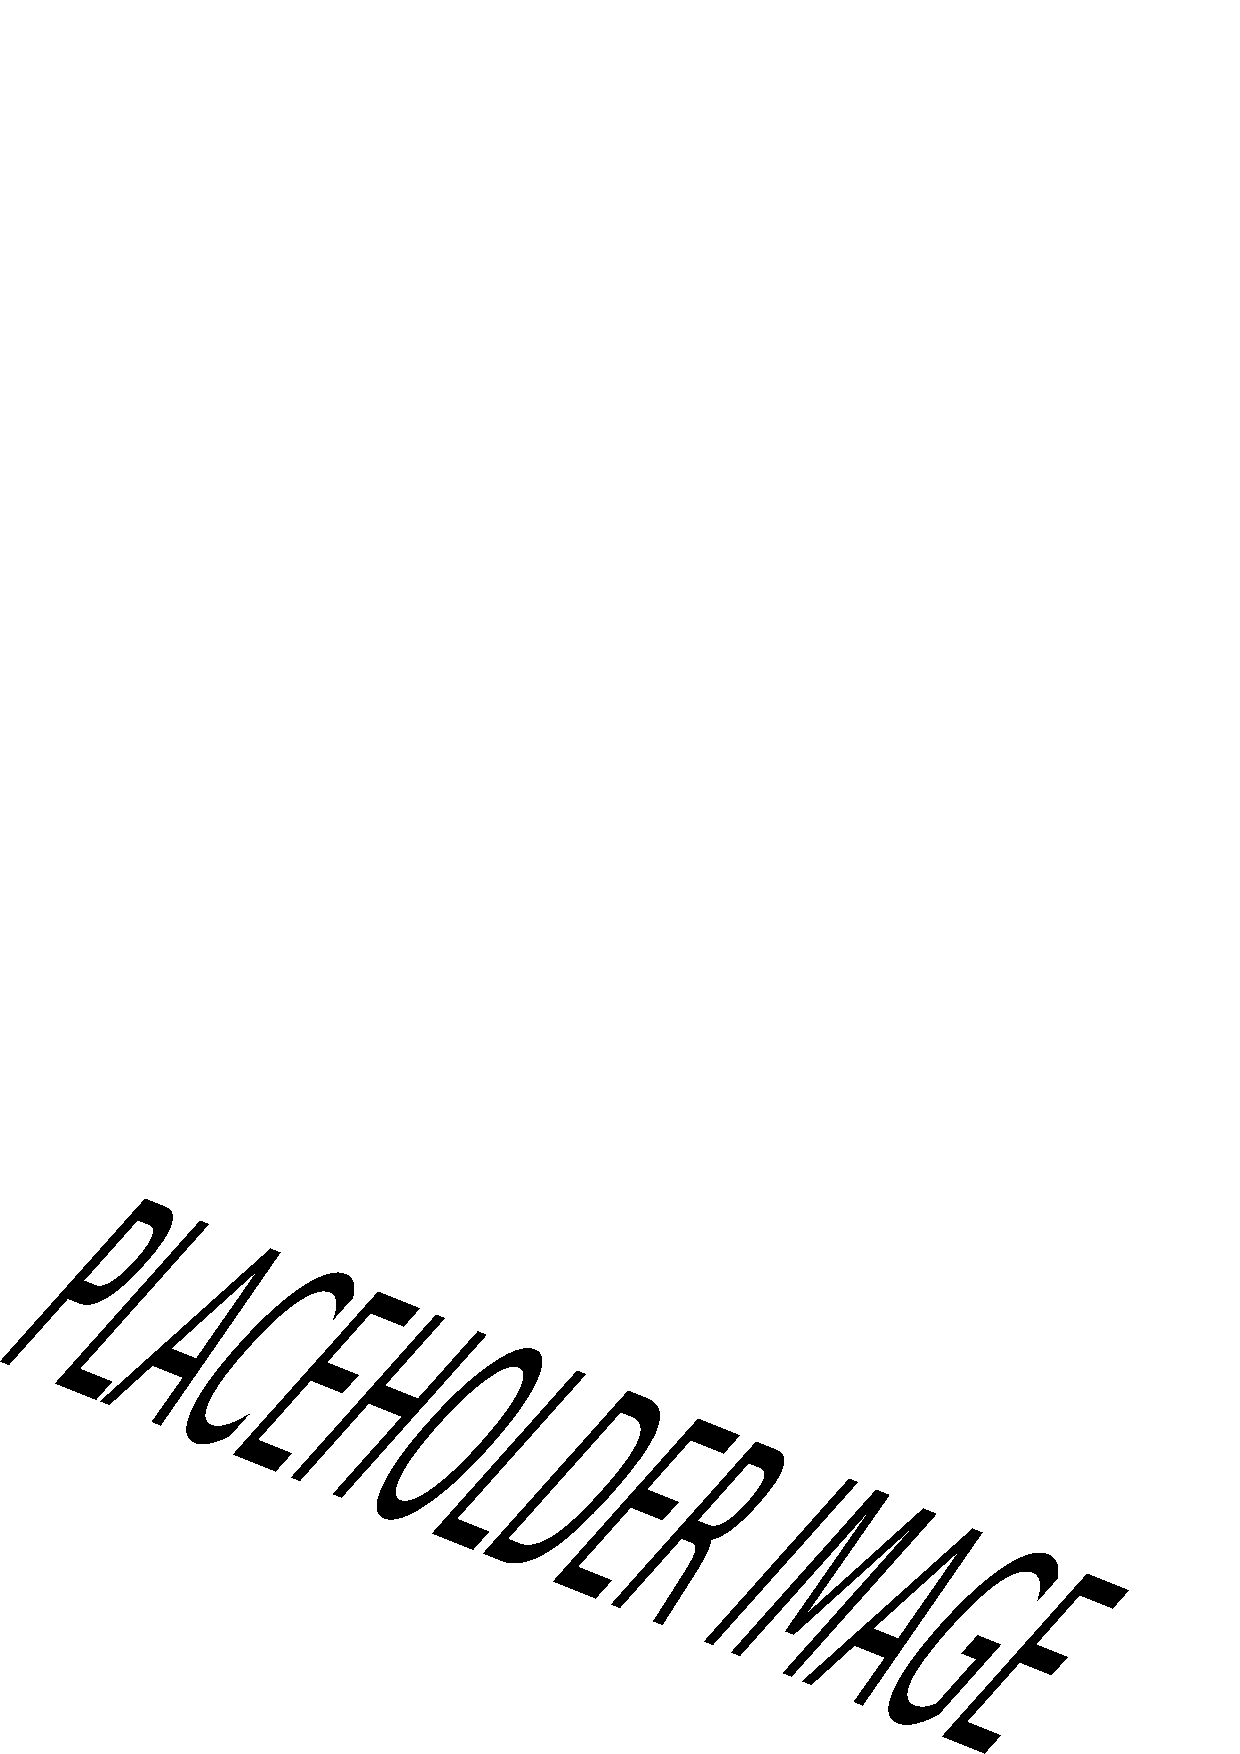
\includegraphics[width=4.0in,height=2.0in]{./pictures/captainplaceholder.png}}
	\caption{Visual particle velocity update \cite{SOSwarm,FundamentalSwarm,CompuIntelligenceIntro,PSOSelfHierarch}}
	%A Particle Swarm Algorithm for Symbols Detection in Wideband Spatial Multiplexing Systems --- Particle movement diagram

	\label{fig:particleVelocityUpdate}
\end{figure}

As discussed in the PSO algorithm overview pbest is the best position the particle has occupied since the start of the algorithm. In the literature there are two defined methods of determining gbest. The most common method used is where gbest is the best position obtained by a particle in the swarm since the start of the algorithm. Thus long term knowledge dictates the best position found which favours exploitation \cite{CompuIntelligenceIntro,FundamentalSwarm}.

With the second method of determining the gbest is the best particle position occupied by any particle in the swarm in the \emph{current} iteration of the algorithm. Thus, short term knowledge dictates the best position found which favours exploration \cite{CompuIntelligenceIntro,FundamentalSwarm}.

As can be observed in equation (\ref{eq:velocityupdate}) the new velocity is added to the old velocity. Therefore, the velocity of particle can get very large, especially for those particles that are far from the pbest and gbest positions. Large velocities are necessary for early exploration, but if the velocity gets too large, the rate at which the particle moves in the solution space is to high and good solutions might be missed \cite{FundamentalSwarm}.

Thus, the velocity of a particle needs to be clamped to ensure it step size stays within acceptable bounds. Equation (\ref{eq:velocityclamp}) is used to clamp the velocity of a particle \emph{before} its position is updated \cite{FundamentalSwarm}.
\begin{align}
	v_i(t+1) &=
	\begin{cases}
	v'_i(t+1), &\text{if $v'_i(t+1) < V_{max}$}\\
	V_{max}, &\text{if $v'_i(t+1) \geq V_{max}$}
	\end{cases} \label{eq:velocityclamp}\\
	V_(max) &= \delta(x_{max} - x_{min})
\end{align}
where $V_{max}$ is the maximum allowed velocity and $\delta \in (0,1]$. The values $x_{max}$ and $x_{min}$ are the respective minimums and maximums of the domain the algorithm is being applied to \cite{FundamentalSwarm}. The value of $\delta$ is very problem dependent and must be carefully chosen as to maximise the exploration - exploitation trade off \cite{FundamentalSwarm}. 

Most of the literature has concentrated on the velocity of the particle as a focal point because it is the main function performing the optimization. In research done by Ratnaweera et. al.\cite{PSOSelfHierarch} a particle positions in the solutions space are continually monitored. If the particle appears to be stagnant in the solution space, the velocity is first updated, and then the particle is reinitialized with a random position. The new position of the particle is then updated with the new velocity. Thus knowledge of the previous discarded particle is retained by using the velocity it had\cite{PSOSelfHierarch}.

In research done by Kalivarapu et al. \cite{PSOPheromones} a PSO algorithm is developed that seeks to incorporate the pheromone notion of ACO algorithms into the velocity updating of particles. The premise of the method is to allow greater sharing of information about promising areas between particles. The algorithm developed by the authors achieved promising results with the algorithm in certain cases finding solutions faster and better solutions than other PSO algorithms \cite{PSOPheromones}. 

Other research done by Monson and Seppi \cite{adaptPSO} is more concerned with how particle presented. In the general PSO algorithm, particles have no physical form or volume, thus particles in the swarm move through each other. The authors changed this in their algorithm by letting each particle have a radius around itself. Therefore, as particles move through the solution space and another particle at a certain time step occupies the same space, the particles are said to collide. As one would expect, when a collision occurs both particles are deflected into random directions \cite{adaptPSO}. At a greater expense of computational time due to constant collision detection, the PSO gains greater exploration in the solution space. 

Finally, in the research by Lenin and Monan a PSO algorithm is developed that is called the Attract and Repulse PSO (ARPSO). The algorithm continually monitors the solutions in the swarm. If the algorithm picks up that a certain percentage of the swarm is stagnating, the algorithm activates the repulse state. In the repulse state particle are repelled from other particles in the swarm, this facilities greater exploration. After a certain number of iterations, the algorithm returns to its default state, where particles attract each other. The attract state facilities exploitation \cite{PSOAttractRepulse}.
\subsubsection{Inertia Weight}
As a object moves with a certain velocity it carries momentum, if the object were to suddenly change direction, momentum would for a certain period still move the article in the previous direction. Inertia weight seeks to add type of behaviour to the particles of the PSO algorithm. It was initially developed to negate the use of clamping a particle velocity. The velocity update equation with added inertia is formulated in equation (\ref{eq:inertia}) \cite{FundamentalSwarm}.
\begin{equation}
v_i(t+1) = wv_i(t) + c_1\phi_{1}(t)[pbest - x_i(t)] + c_2\phi_{2}(t)[gbest - x_i(t)]\label{eq:inertia}
\end{equation}
The addition of inertia ($w$ in equation (\ref{eq:inertia}) to the general velocity update equation is simple and elegant which is why it has been adapted to a wide variety of PSO algorithms. The inertia value allows one to control the amount of control the social and cognitive components have with regard to velocity updates \cite{FundamentalSwarm}. 

For values of $w$ that are greater than 1, a large amount of momentum is preserved as the particles velocity are updated and hence, the particle explores more \cite{FundamentalSwarm}. When $w < 1$, each time the particle updates it velocity is loses a certain amount of momentum, hence, the particle seems to slow down allowing it to exploit the current solution space in finer detail \cite{FundamentalSwarm}.

Even though inertia was developed to remove the use of velocity clamping, it did not entirely achieve its goal. For values of $w$ that are greater than 1, the particle keeps a lot of momentum and accelerates even more. Therefore, as the particle accelerates its step size through the solution space gets larger and larger, increasing the probability that it will miss a good solution. This disadvantage is only applicable for algorithms that keep the inertia value static \cite{CompuIntelligenceIntro,FundamentalSwarm}.

To allow for a greater trade-off between exploration and exploitation, the inertia value was made dynamic. Exploration is favoured early on in a optimization algorithm and in return exploitation is favoured later on the algorithm when it is near a optimum. Thus, various methods linear decreasing and non-linear decreasing and have been developed that modify the inertia component as the algorithm moves around in the solution space \cite{CompuIntelligenceIntro,FundamentalSwarm}.

Finally, a similar inertia type component was developed from the analyse of particle dynamics \cite{FundamentalSwarm}. This new component is called the \emph{constriction coefficient} and like the inertia above, also modifies the velocity update equation slightly\cite{adaptPSO,FundamentalSwarm,CompuIntelligenceIntro}. 

This modification can be observed in equation (\ref{eq:velocityconstriction}) which is the standard velocity equation with the constriction coefficient. The constriction coefficient is formulated in equation (\ref{eq:constriction})\cite{adaptPSO,FundamentalSwarm,CompuIntelligenceIntro}.
\begin{align}
v_i(t+1) &= \chi[v_i(t) + c_1\phi_{1}(t)[pbest - x_i(t)] + c_2\phi_{2}(t)[gbest - x_i(t)]]\label{eq:velocityconstriction}\\
\chi &= \frac{2\kappa}{\lvert 2 - \phi - \sqrt{\phi^2 - 4\phi}\rvert}\label{eq:constriction}
\end{align}

The constriction coefficient is represented by the value $phi$ and allows one to omit the usage of velocity clamping. The constriction coefficient evaluates to a ever decreasing value between $[0,1]$. By using the constriction coefficient the PSO algorithm is also guaranteed to converge for values of $phi \geq 4$ and $\kappa \in [0,1]$. As with the inertia discussed above, high values of $\kappa$ allows for greater exploration and slow convergence. Where as low values of $\kappa$ forces the algorithm to exploit the solution space and converge quickly \cite{adaptPSO,FundamentalSwarm,CompuIntelligenceIntro}.
\subsection{PSO on the FAP}
The PSO algorithm is also a relatively new algorithm and has been applied to only a handful of NP-Complete problems which includes the FAP. In this dissertation the PSO algorithm will be utilized on the FS-FAP to try and produce optimal solutions. 

In the literature only two groups have presented research where the PSO has been applied on the FAP to produce an near optimal solution. The research presented by these groups concentrate on the MS-FAP variant of the FAP. Thus, the aim of their algorithm is to reduce the span of frequencies used, where as the problem this dissertation is concerned with is the FS-FAP where the amount of interference generated needs to be minimized. 

To date, no PSO algorithm has been presented which has been designed to operate on the FS-FAP variant of the FAP. Therefore, the interest in the research presented is more to do with how the authors went about encoding a particular frequency plan as a position for a particle, than with the actual optimization procedure.

A general overview of the work produce by these groups will now be presented.

In the research presented by Elkamchouchi et. al\cite{EgyptFAPPSO} a PSO algorithm is applied to produce optimal solutions for the MS-FAP. The way the authors went about to assign frequencies in their algorithm is known as the Frequency Exhaustive Assignment (FEA).
This method works by first generated a list of calls, called a \emph{call list} denoting calls that occur in the system\cite{EgyptFAPPSO}. 

The method then iterates over the calls in the list and assigns the lowest possible frequencies to the calls without violating interference constraints\cite{EgyptFAPPSO}. The authors note that the specific frequency that is assigned to a particular call depends heavily on the order the calls are in the list\cite{EgyptFAPPSO}.


\section{Summary}
In this chapter a discussion was given on three swarm intelligence algorithms. The first section presented a discussion on the Ant Colony Optimization Algorithm.

The general flow of the algorithm was presented with the help of a diagram (see figure \ref{fig:ACOAlgorithmFlowChart}) as well as an explanation with regard to how the algorithm came about and the basic flow of the algorithm. The defining characteristics of the algorithm was also discussed. The discussion on the ACO algorithm concluded with a literature review of the ACO being applied to the FAP.

The second section that was presented provided an overview of the Artificial Bee Colony Optimization Algorithm. A discussion was presented on how the algorithm was developed and how the algorithm performs its search in a problem space. A diagram was also presented that outlines the general flow of the ABC algorithm.

Also within the second section, a series of defining characteristics are presented and explained. Each characteristic is a defining attribute of the algorithm that makes it unique with regard to other algorithms. No literature study was presented on the algorithm being applied on the FAP since to date, no research has been presented of such a ABC algorithm.

This chapter concluded with a discussion on the most important algorithm. The algorithm this dissertation will be using to apply it to the FAP, namely the Particle Swarm Optimization algorithm. In the last section how the algorithm was developed was discussed as well as the general flow of the algorithm when search the problem space.

A diagram depicting the flow of the PSO algorithm was also presented(see figure \ref{fig:PSOAlgorithmFlowChart}). Futhermore, characteristics that make the algorithm unique were explained. The final section of this chapter concluded with a literature review of the PSO algorithm being applied to the FAP.
